\documentclass{beamer}
\usepackage{setspace}
\usepackage{bm,color,float,epstopdf,amsthm,epstopdf}
\usepackage{multirow,tikz}
\newcommand{\fttheory}[1]{\fcolorbox{blue}{blue}{\color{white}\textbf{#1}\hspace{\textwidth}}}
\newcommand{\ftexampl}[1]{\fcolorbox{orange}{orange}{\color{black}\textbf{#1}\hspace{\textwidth}}}
\newcommand{\ftdata}[1]{\fcolorbox{violet}{violet}{\color{white}\textbf{#1}\hspace{\textwidth}}}
\newcommand{\ftheader}[1]{\fcolorbox{lightgray}{lightgray}{\color{black}\textbf{#1}\hspace{\textwidth}}}
\newcommand{\ftvocab}[1]{\fcolorbox{cyan}{cyan}{\color{black}\textbf{#1}\hspace{\textwidth}}}
\newcommand{\usd}{\text{ {\scriptsize USD}}}
\newcommand{\eur}{\text{ {\scriptsize EUR}}}
\newcommand{\aud}{\text{ {\scriptsize AUD}}}
\newcommand{\mxn}{\text{ {\scriptsize MXN}}}
\newcommand{\musd}{\text{ m {\scriptsize USD}}}
\newcommand{\meur}{\text{ m {\scriptsize EUR}}}
\newcommand{\maud}{\text{ m {\scriptsize AUD}}}

\renewcommand{\arraystretch}{1.5}
\begin{document}

%-----------------------------------------------------------------------------%
% forward
\begin{frame}{\ftheader{Fowards}}
	\begin{itemize}
		\item In this lecture, we begin our study of derivatives 
		\item We will start with \textit{forwards} 
		\item Standardized implementations of forwards are called \textit{futures}
		\item We will then use forwards to study\\
			(1) swaps\\ 
			(2) exchange rates
		\item Read Satyajit Das's book \textit{Traders, Guns, \& Money}
	\end{itemize}
\end{frame}

%-----------------------------------------------------------------------------%
% vocabulary
\begin{frame}{\ftvocab{Vocabulary}}
	\begin{itemize}
		\item A \textit{counterparty} is a trader with whom one trades
		\item A \textit{derivative} is a security for which the payoff depends on the payoff of other securities (called \textit{underlying} securities)
		\item A \textit{forward} is a contract that specifies the date and price at which one trader buys a security from another (the date is called the \textit{maturity} and the price is called the \textit{forward price}) 
		\item The \textit{spot price} is the market price of the security 
		\item The \textit{basis} is the difference between the forward and spot prices 
	\end{itemize}
\end{frame}

%-----------------------------------------------------------------------------%
% strategies
\begin{frame}{\fttheory{Forward Mechanics}}
	\begin{itemize}
		\item The trader who is long ``buys'' the forward and must buy the underlying security from her counterparty at the forward price at maturity
		\item The trader who is short ``sells'' or ``writes'' the forward and must sell the underlying security to her counterparty at the forward price at maturity
		\item \textit{Physical settlement} occurs when the long and short traders exchange ownership  of the security, where \textit{cash settlement} occurs when they exchange the cash value of the security instead of ownership of the security itself 
		\item Since positions are settled at maturity, there is no initial cash flow: everything happens ``in the future''
    \end{itemize}
\end{frame}

%-----------------------------------------------------------------------------%
% payoffs
\begin{frame}{\fttheory{Forward Payoffs}}
    \begin{center}
        \begin{tabular}{cc}
            Long Forward: $S-K$ & Short Forward: $K-S$ \\
            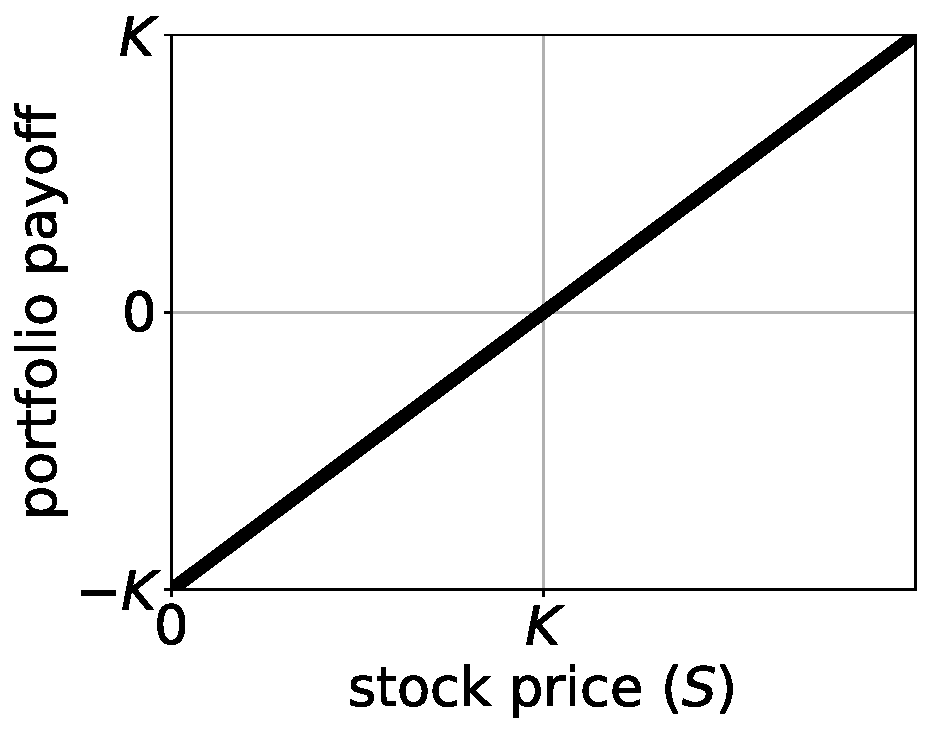
\includegraphics[scale=.3]{longforward} & 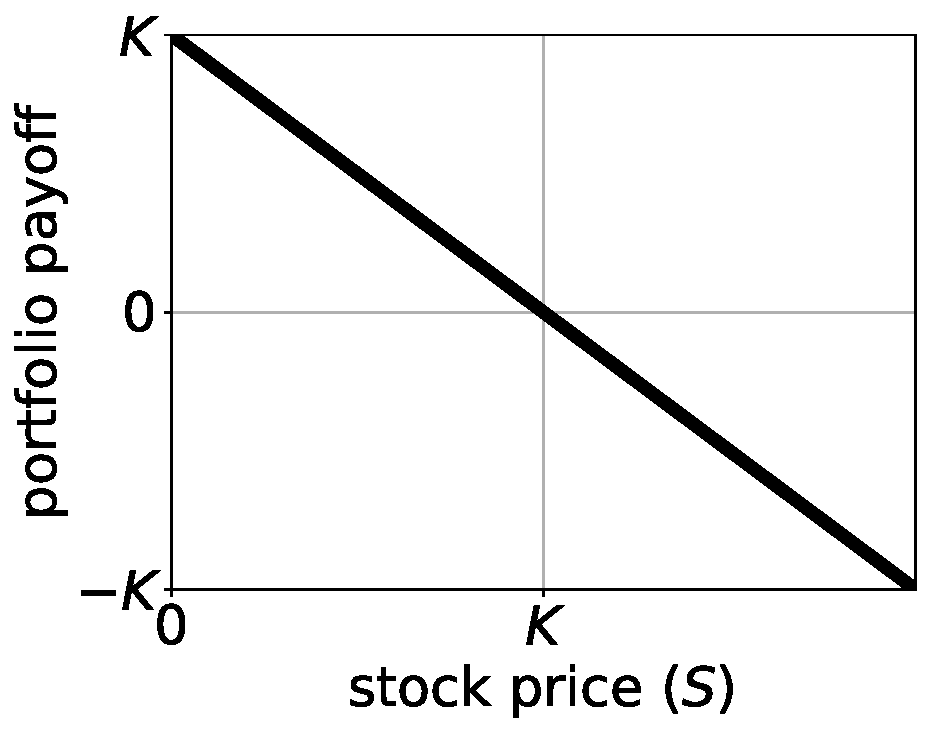
\includegraphics[scale=.3]{shortforward}
        \end{tabular}
    \end{center}
	\begin{itemize}
		\item $S$ is the spot price at maturity and $K$ is the forward price.
		\item Long trader buys underlying for $K$ from short trader, sells for $S$ to market, and makes $S-K$ (bullish)
		\item Short trader buys underlying for $S$ from market, sells for $K$ to long trader, and makes $K-S$ (bearish)
	\end{itemize}
\end{frame}

%-----------------------------------------------------------------------------%
% payoffs
\begin{frame}{\ftexampl{\hypertarget{frame:payoffs1}{Forward Payoffs: Problem 1}}}
	\textbf{Problem.} Apple (AAPL) is trading for (about) $270\usd$ a share. James Simons (Renaissance Technologies) writes (sells) a five-year forward contract with a forward price of $300\usd$ to Ray Dalio (Bridgewater). What are the obligations-of and payoffs-to each of the traders if the spot price is (1) $310\usd$ or (2) $290\usd$ at maturity?\\ 
\vfill
	\textbf{Solution.} Simons is obligated to sell Apple shares to Dalio at $300\usd$ a share. If the spot price in three-years is $310\usd$, then Simons buys Apple shares in the market for $310\usd$ and then sells them to Dalio for $300\usd$ at a loss of $10\usd$. Dalio buys the shares from Simons for $300\usd$ and then sells them in the market for $310\usd$ at a profit of $10\usd$. If the price in three-years is $290\usd$, then the losses/profits just flip: Simons gains $10\usd$ and Dalio loses $10\usd$. Rather than deal with the shares, Simons can just pay Dalio (or Dalio Simons) $10\usd$. 
\end{frame}

%-----------------------------------------------------------------------------%
% corporate applications: a vignette
\begin{frame}{\fttheory{Corporate Applications: a Vignette}}
	\begin{itemize}
		\item Consider an oil company and an airline.  
		\item How much will the price of oil be in the future, when they are ready to sell the oil they produced?  
		\item The revenue of this company depends on oil prices, which are extremely volatile.
		\item The airline has a problem that mirrors that of the oil production company. 
		\item How can forwards help these two firms?
	\end{itemize}
\end{frame}

%-----------------------------------------------------------------------------%
% corporate applications: a vignette
\begin{frame}{\fttheory{Corporate Applications: a Vignette}}
	\begin{itemize}
		\item The two firms can enter into an agreement today that specifies the price at which the oil producer sells the oil to the other company in the future. 
		\item Such an agreement will reduce the source of risk for both parties!  
		\item The oil producer delivers oil at a price agreed upon now, regardless of the market price at the time when oil is produced. 
		\item This requires that both parties be willing to lock in the price to be paid or received for delivery of the commodity. 
		\item This can be achieved using forwards.
	\end{itemize}
\end{frame}

%-----------------------------------------------------------------------------%
% corporate applications
\begin{frame}{\ftdata{Corporate Applications}}
    \begin{center}
        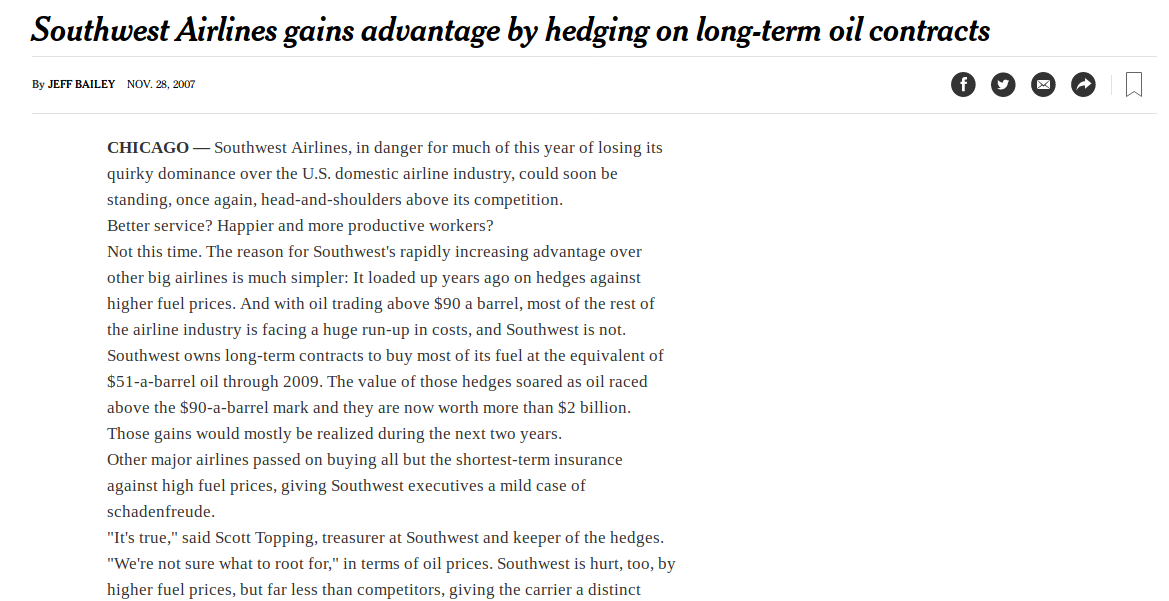
\includegraphics[scale=.3]{swa}
    \end{center}
\end{frame}

%-----------------------------------------------------------------------------%
% pricing new forwards
\begin{frame}{\fttheory{Spot-Futures Parity}}
\begin{itemize}
	\item $T$ is the term, $S_{0}$ is the spot price on date $0$, $S_{T}$ is the spot price on date $T$, and $K$ is the forward price
    \item Spot-Futures Parity 
\end{itemize}
    \begin{center}
        \begin{tabular}{lccc}
            Security & Q & CF$_{0}$ & CF$_{T}$ \\ \hline
            Forward & 1 & 0 & $S_{T}-K$ \\ \hline\hline
            Stock & 1 & $-S_{0}$ & $S_{T}$ \\
			Risk-Free & $-K/(1+r_{F})^{T}$ & $K/(1+r_{F})^{T}$ & $-K$ \\ \hline
			& & $-S_{0}+K/(1+r_{F})^{T}$ & $S_{T}-K$
        \end{tabular}
    \end{center}
	\begin{equation}
		\boxed{K\overset{\text{``should''}}{=}S_{0}(1+r_{F})^{T}}
	\end{equation}
\end{frame}

%-----------------------------------------------------------------------------%
% pricing new forwards
\begin{frame}{\ftexampl{\hypertarget{frame:spotfuturesparityhedging}{Spot-Futures Parity: Hedging Problem}}}
	\textbf{Problem:} Consider again Simons and Dalio. Suppose that the annually compounded risk-free rate is 2.1296\%. What should the forward price $K$ be? How does Simons hedge the position?\\
\vfill
 \textbf{Solution:} The forward price is
	\begin{equation}
		K=S_{0}(1+r_{F})^{T}=(270\usd)(1+.021296)^{5}=300\usd
	\end{equation}
	In order to hedge his short position in the forward, Simons can buy Apple stock by borrowing $270\usd$ at the risk-free rate. At maturity, he can sell his shares to Dalio for $300\usd$ and repay his loan (the balance of which has grown to $300\usd$).
\end{frame}

%-----------------------------------------------------------------------------%
% pricing new forwards
\begin{frame}{\ftexampl{\hypertarget{frame:spotfuturesparitymargin}{Spot-Futures Parity: Margin Problem}}}
	\textbf{Motivation.} In practice, both traders must post margin because both are exposed to losses. Margin requirements are computed using the forward price. For futures, profits and losses are \textit{marked-to-market} (credit profits to margin account, debit losses).
	\vfill
	\textbf{Problem.} 
	\begin{enumerate}
		\item If the initial margin requirement is 20\%, how much margin (USD) must Simon and Dalio post? What are Simon's and Dalio's returns be if Apple falls the next morning to $261\usd$ (ignoring compounding effects)?
		\item What if the initial margin requirement is 10\%?
	\end{enumerate}
\end{frame}

%-----------------------------------------------------------------------------%
% pricing new forwards
\begin{frame}{\ftexampl{Spot-Futures Parity: Margin Problem}}
	\textbf{Solution.} 
	\begin{enumerate}
		\item The forward price is $300\usd$, so Simon and Dalio must post $60\usd$. If Apple falls to $261\usd$ (a decline of about 3.33\%), the new forward price is
		\begin{equation}
			K=S_{0}(1+r_{F})^{T}=(261\usd)(1+.021296)^{5}=290\usd
		\end{equation}
			The forward price falls by $10\usd$, so Simon's margin grows from $60\usd$ to $70\usd$ (a return of 16.67\%) while Dalio's margin falls from $60\usd$ to $50\usd$ (a return of -16.67\%). 
		\item If the margin requirement is 10\%, then Simon's return is 33.33\% and Dalio's return is -33.33\%.  
	\end{enumerate}
\end{frame}

%-----------------------------------------------------------------------------%
% pricing existing forwards
\begin{frame}{\fttheory{Pricing Existing Forwards}}
   \begin{itemize}
	   \item Forwards, like all of the derivatives we will study, can be sold in a secondary market
       \item Suppose you go long a forward that expires in \underline{two} years.
       \item Step forward one year. 
       \item Consider a new forward that expires in \underline{one} year.
       \item How much could you sell your old forward for (say $f_{0}$)? 
	   \item This is the problem of pricing an existing forward
   \end{itemize}
\end{frame}

%-----------------------------------------------------------------------------%
% pricing existing forwards
\begin{frame}{\fttheory{Pricing Existing Forwards}}
    How do you price anything? Build a replicating portfolio!
    \begin{center}
        \begin{tabular}{lcc}
            Security & CF$_{1}$ & CF$_{2}$ \\ \hline
            Old Forward ($K_{0}$) &  $-f_{0}$ & $S_{2}-K_{0}$ \\ \hline
            \multicolumn{3}{c}{Replicating Portfolio} \\ \hline
			New Forward ($K_{1}$) & $0$& $S_{2}-K_{1}$ \\ 
			Risk Free &  $-(K_{1}-K_{0})/(1+r_{F})$ & $K_{1}-K_{0}$ \\ \hline
			& $-(K_{1}-K_{0})/(1+r_{F})$ & $S_{2}-K_{0}$
        \end{tabular}
    \end{center}
    \begin{equation}
		\boxed{f_{0}\overset{\text{``should''}}{=}\frac{K_{1}-K_{0}}{1+r_{F}}}
    \end{equation}
\end{frame}

%-----------------------------------------------------------------------------%
% pricing existing forwards: problem 1
\begin{frame}{\ftexampl{\hypertarget{frame:pricingexistingforwards1}{Pricing Existing Forwards: Problem 1}}}
	\textbf{Problem.} Suppose that the spot price was $S_{0}=100\usd$ a year ago and is $S_{1}=105\usd$ today. What is the forward price of a two-year forward written a year ago? Suppose that the annually compounded risk-free rate is $r_{F}=1.5\%$\\
	\vfill
	\textbf{Solution.}
	\begin{itemize}
        \item The old and new forward prices are 
            \begin{align}
				K_{0}&=S_{0}(1+r_{F})^{2}=103.0225\usd\\
				K_{1}&=S_{1}(1+r_{F})=106.5750\usd
            \end{align}
        \item The old forward trades now trades for
            \begin{equation}\small
				f_{0}=\frac{K_{1}-K_{0}}{1+r_{F}}=\frac{106.5750\usd-103.0225\usd}{1+.015}=3.50\usd
            \end{equation}
    \end{itemize}
\end{frame}

%-----------------------------------------------------------------------------%
% pricing existing forwards: problem 2
\begin{frame}{\ftexampl{\hypertarget{frame:pricingexistingforwards2}{Pricing Existing Forwards: Problem 2}}}
	\textbf{Problem.} What if the spot price is $S_{1}=101.5\usd$ today?
	\vfill
	\textbf{Solution.}
    \begin{itemize}
		\item The old and new forward prices are 
            \begin{align}
				K_{0}&=S_{0}(1+r_{F})^{2}=103.0225\usd\\
				K_{1}&=S_{1}(1+r_{F})=103.0225\usd
            \end{align}
        \item The old forward trades for
            \begin{equation}\small
				f_{0}=\frac{K_{1}-K_{0}}{1+r_{F}}=\frac{103.0225\usd-103.0225\usd}{1+.015}=0\usd
            \end{equation}
    \end{itemize}
\end{frame}
\end{document}
